%% $RCSfile: proj_report_outline.tex,v $
%% $Revision: 1.3 $
%% $Date: 2016/06/10 03:41:54 $
%% $Author: Mayur Panchal$

\documentclass[11pt
              , a4paper
              , twoside
              , openright
              ]{report}


\usepackage{float} % lets you have non-floating floats

\usepackage{url} % for typesetting urls

\usepackage{xspace} % space after trademarks specifically

\usepackage{pdfpages}

\usepackage{listings}

\let\OldTexttrademark\texttrademark
\renewcommand{\texttrademark}{\OldTexttrademark\xspace}%
\setlength{\parskip}{1em}

%
%  We don't want figures to float so we define
%
\newfloat{fig}{thp}{lof}[chapter]
\floatname{fig}{Figure}

%% These are standard LaTeX definitions for the document
%%                            
\title{Network switching fabric for Gigabit links}
\author{Mayur Panchal}

%% This file can be used for creating a wide range of reports
%%  across various Schools
%%
%% Set up some things, mostly for the front page, for your specific document
%
% Current options are:
% [ecs|msor|sms]          Which school you are in.
%                         (msor option retained for reproducing old data)
% [bschonscomp|mcompsci]  Which degree you are doing
%                          You can also specify any other degree by name
%                          (see below)
% [font|image]            Use a font or an image for the VUW logo
%                          The font option will only work on ECS systems
%
\usepackage[image,ecs]{vuwproject}

% You should specifiy your supervisor here with
%     \supervisor{Firstname Lastname}
% use \supervisors if there is more than one supervisor

\supervisors{Bryan Ng, Robin Dykstra}

% Unless you've used the bschonscomp or mcompsci
%  options above use
%   \otherdegree{OTHER DEGREE OR DIPLOMA NAME}
% here to specify degree

\otherdegree{Bachelor of Engineering with Honours in Electronic and Computer Systems Engineering}

% Comment this out if you want the date printed.
\date{}

\begin{document}

% Make the page numbering roman, until after the contents, etc.
\frontmatter

%%%%%%%%%%%%%%%%%%%%%%%%%%%%%%%%%%%%%%%%%%%%%%%%%%%%%%%

%%%%%%%%%%%%%%%%%%%%%%%%%%%%%%%%%%%%%%%%%%%%%%%%%%%%%%%

%\begin{abstract}

%A short description of the project goes here.

%\end{abstract}

%%%%%%%%%%%%%%%%%%%%%%%%%%%%%%%%%%%%%%%%%%%%%%%%%%%%%%%

\maketitle

%\chapter*{Acknowledgments}\label{C:ack} 
Any acknowledgments should go 
in here, between the title page and the table of contents.  The 
acknowledgments do not form a proper chapter, and so don't get a 
number or appear in the table of contents.

\tableofcontents

% we want a list of the figures we defined
\listof{fig}{Figures}

%%%%%%%%%%%%%%%%%%%%%%%%%%%%%%%%%%%%%%%%%%%%%%%%%%%%%%%

\mainmatter

%%%%%%%%%%%%%%%%%%%%%%%%%%%%%%%%%%%%%%%%%%%%%%%%%%%%%%%

% individual chapters included here
\chapter{Introduction}\label{C:intro}

Fast internet connections are becoming more and more desired as high bandwidth media consumption and internet-based services grow in popularity. The speed of an internet connection can be separated into two distinct metrics,
latency, and bandwidth. Latency is the time taken for information to travel from one place to another and the delay
introduced by the device itself, while bandwidth is the amount of information that can flow reliably from end to end.
When a user is accessing a website, such as Facebook, their requests traverse multiple network devices (physical
hardware) to reach that website's servers. Throughout this travel, each network device introduces some latency, as
there is processing time required to send information to the right destination. Although this delay is very small,
over the course of multiple hops it can become significant. Measuring this small latency with current solutions is
convoluted and without the right systems, can be unreliable. By measuring this latency, we can enable research to
reduce latency to create a faster internet.

\section{Problem}

There have been studies dedicated to the reduction of latency. Some ways to reduce this latency include making “smart” network routers \cite{smartrouters} and low latency wireless systems \cite{5g}. 
This research is reaching the point where network traffic can have latency as little as 1ms \cite{lessthan1ms} or 
below. To advance further, new tools need to have the capability of measuring this latency.

Existing hardware solutions to measuring latency are capable of measuring less than 1 ms but require some additional training in the software suite provided with the hardware \cite{dagfeatures}. Additional processes attached
to hardware-based methods can require dedicated computers for the measurement and analysis of networks. This means
that each researcher would require an understanding of the software suite accompanied with a dedicated computer
all setup for specific tests to be run. Each different test would require reconfiguring of both hardware and software.
This drives the cost of using the device up, in terms of both time and money.

Current software solutions can measure latency in ethernet network traffic down to a resolution of
milliseconds and sometimes microseconds \cite{pingisbad}. There are no software solutions that can measure
latency in the order of nanoseconds reliably \cite{timeinlinux}. Measuring the latency in nanoseconds is needed as network switches have very low latency and the time between ingress and egress can range from
microseconds to nanoseconds. If it could be measured accurately, then analysis could be performed
on network traffic through network switches to research new ways to reduce latency.

Existing methods to measure latency within microseconds and nanoseconds require monolithic devices which need
setting up and installing device drivers, proprietary software, or even a replacement of existing hardware systems.
Once set up, these devices often require data conversion of results to be compatible with data analysis methods and
evaluation programs. Occasionally these programs are embedded within in manufacturers software, but the user is
limited to what the manufacturer has chosen as relevant outputs for the user. These can be useful most of the time,
but occasionally the user would need to export the data to another data analysis tool they are familiar with for
further processing. This inflexibility is prominent in many high-end network performance analysis tools, causing delays in retrieving test results for evaluation.

A reduction in network latency would be a huge boon to future technologies. For example, less
latency in video streaming can enable doctors from remote locations to perform surgery with
minimal lag between actions and responses \cite{remotesurgery}. The stock market is another example of improvement with this technology, as less latency ensures that stock market trade deals can be completed faster.

\begin{quote}
    \centering
    ``We are running through the United States with dynamite and rock saws, so that an algorithm can
    run three microseconds faster.`` \em --- Kevin Slavin, How Algorithms shape our world \cite{tedTalkAlgorithms}
\end{quote} 

\par Many improvements made at a nanosecond scale can add up to microseconds or even milliseconds of latency
reduction. Improvements cannot be done without knowing how much this can improve by without the tools to measure it.

A software-based approach has the limitation that the timing functions must be processed by a
Central Processing Unit (CPU) \cite{CPUtiming}. This means the counters for timing functions could be offset from 
the true value. Higher resolution latency measurements can be achieved through a hardware implementation of a packet
timer. This circumvents the limitations of a software-based approach.

\section{Solution}

Latency occurs the instant that a network packet is sent from a computer. The processing times for the network packet
to flow through the networking stack in the operating system can be considered a constant unavoidable delay which is
not in the scope of this project.

Because the nature of when the latency occurs, it would be best measured by considering the raw electronic signals 
from the ethernet port on the device to ensure there is no operating system lag. To achieve this, microcontrollers, 
discrete logic gates, and a Field Programmable Gate Array could be implemented. A microcontroller could be used but 
then the same issues arise, that a CPU clocking through instructions would deviate the true timing counter value. 
Another approach would be to use discrete logic gates to measure the timing accurately, but this will become 
complicated very rapidly, and propagation delays through discrete devices would reduce the accuracy. Hence the 
preferred choice is to implement the packet latency measurement unit on a Field Programmable Gate Array (FPGA). More 
information about FPGA’s is in the Background section of the report. This way complex digital designs can be 
simplified down to a simple set of blocks, and there is no overhead that a processor would introduce. The drawback 
to using an FPGA is that the learning curve to developing on the platform is quite steep, and also communication 
with existing systems is difficult and is usually aided by the use of a microcontroller (such as an ARM or x86 based 
co-processor)

\par This report will focus on the work done so far in implementing an FPGA based packet latency timing
device. This project is limited to Ethernet-based networks as they are most widely used \cite{etherneteverywhere}.
The next section describes some key concepts around the problem, with some examples of current implementations of the
solution. Following that will by the approach taken to design the FPGA based device beginning with hardware choices
made and the details of what the final implementation would look like. After, the implementation details of the 
project are presented and an explanation of the work that took place. This work is evaluated and the results are then
concluded. The final part is the improvements that can be applied to the minimum viable product, with a conclusion of
the project as a whole.

\chapter{Background and Related Work}\label{C:back}

\section{General Networking}

Information which is sent across a network is generally divided into smaller pieces. When each piece
traverses a network, extra information is repeatedly added and removed until it has arrived at the
destination. This extra information is split into multiple layers and each layer has a different function.
The Open Systems Interconnection (OSI) model (Figure: \ref{fig:OSIModel}) is a widely implemented standard that
defines these different layers of extra information and their purpose.

\begin{figure}[H]
    \begin{center}
        \includegraphics[width=5cm,height=5cm,keepaspectratio]{Images/OSIModel.png}
        \caption{OSI Model \cite{OSIPic}}
        \label{fig:OSIModel}
    \end{center}
\end{figure}

Network switches and network routers interpret the destination based off information found in
Layer 2 or Layer 3 from the OSI model, hence I must adhere to the protocol standards found at these
layers. Layers 4 and above provide other benefits to the payload such as reliability and is not a
concern for this project.

\subsection{Layer 1}

In Ethernet systems, Layer 1 refers to the physical medium that information is being sent over.
Gigabit ethernet based systems use a copper wire as the physical medium, with electrical voltages
representing the information. For this project, the latency is measured at this layer.

\subsection{Layer 2}

Layer 2 is responsible for transferring data between adjacent network devices \cite{IEEE802}. This is important as
information will be flowing to and from adjacent nodes, through a switch or router. To ensure that
information flows through the switch or router, this layer must be taken into consideration to ensure
successful transmission and reception of information.
This layer is important to the project as the measuring device will be timing the latency between adjacent 
network devices and through network switches, both of which rely on Layer 2 information.

\subsection{Layer 3}

Information from one hop to another is determined by the Layer 3 protocol. This ensures that
information is correctly routed to the destination from the source. This layer is important as the
information stored at this layer ensures the correct path is taken from sender to receiver. This is
different to Layer 2, as this can incorporate non-adjacent nodes as well.

\section{Latency Definitions}

For this project, latency in a network will be defined in the following ways. 
This project will be focusing on One Way Trip time, because it is a subset of the other latencies.

\subsection{Connection Time}

Connection time describes the time that two devices take to enable information flow between them. In
some cases, there are many synchronisation and authentication steps that need to take place before
any information can flow. This latency is defined as the initialization of the first command, to the
processing of the final command.

\subsection{Return Trip Time}

In some cases, the return trip time can be used to measure the one-way latency of two devices. One
device sends a request for an echo and when the echo is recieved, the time taken from transmition to reception is
twice the latency between devices.

\subsection{One way Trip Time}

This is similar to Return Trip Time but instead of requiring an echo back to the sender, the receiver is on the
same device. Hence the latency of the connection is measured as the time taken for the information
to flow from one port on the device to another.

\section{Current Solutions}

There are solutions present which can measure latency to a high degree (< 1 ms) but have some drawbacks in different areas.
These can be split into two different catagories, hardware and software, referring to the process of which they measure latency.

\subsection{Software}

\subsubsection{Ping}

Ping is a Linux utility that can be used to estimate the latency to a given network server. 
This is for large distance measurements, as the accuracy of this ranges from seconds to milliseconds. 
It has also been tested that this utility is unreliable for performance extensive testing as momentary ‘glitches’ 
can appear in networks, causing random and unpredictable results \cite{pingisbad}.
It is very useful at measuring very large latencies (>1 milliseconds) and displaying them in a concise format 
for analysis by the user. 
This does not meet the need of having the ability to measure time in the nanosecond range, but a useful takeaway 
is to make sure that values are presented in an easy to analyse format (printing to screen, or to a file).

\subsubsection{Data plane Development Kit (DPDK)}

DPDK is a software implementation of rapid packet processing. 
This software utilises low level software drivers to interact directly with the hardware. 
Doing so requires specific hardware on the computer which needs to be compatible with the software itself.
Reducing the packet processing time reduces the time offset created by the CPU, but not fully removes it. 
Examples in the source code have shown that the timing value is dependent on CPU frequencies \cite{dpdkcode} 
and Dynamic Frequency scaling \cite{turboboost} of modern CPUs can cause a change in this frequency at any time.
An advantage of this solution is that it can produce a high-resolution time value (in the order of nanoseconds) 
and is easily accessible by a user in software for processing and analysing. 
A lesson learnt from this approach is that a CPU based system for measuring high resolution timers will not be precise or accurate.

\subsubsection{PF\textunderscore RING}

Another software solution is PF\textunderscore RING by ntop\texttrademark. 
It is a rapid packet processing library that does not require the need for specific hardware.  
PF\textunderscore RING allows for more efficient packet capturing and filtering by utilising more cores and threads on a CPU \cite{pfringworks}.
This library is more focused on throughput of packets processed rather than latency. 
This is less accurate than the DPDK but increases the flexibility of the platform it can implemented on. 
As with all software based approaches, this does not meet the requirements of being able to measure time in nanoseconds reliably.
An insight from this approach is to flexibility of platform is good for users but will not be a requirement for this project.

\subsection{Hardware}

\subsubsection{Data Acquisition and Generation (DAG) 10x2-S}

\par The DAG 10x2-S by Endace is a hardware based packet capturing solution with high precision nanosecond scale precision \cite{dagprecision}. 
This is a physical device which connects to a x86 based computer and communicates via Peripheral Component Interconnect Express (PCIe). 
The DAG 10x2-S is recommended for capturing network packets over gigabit ethernet links, as the other models cost more and have other unnecessary features \cite{dagfeatures}.
It is an expansion card for a computer which extends the capabilities of the computer to accurately capture and timestamp packets to a high degree. 
This device has the capabilities to timestamp packets with a resolution of 4ns \cite{dagprecision}. 
This meets all the requirements of the project but is very costly (\$2500 USD \cite{dagprice}) and methods for obtaining a device can only be done through Endace themselves. 

\subsubsection{Field Programmable Gate Array (FPGA)}

\par A FPGA is an array of configurable logic gates. The number of gates are in the order of thousands to
millions. This many configurable gates allows for complex logical structures and digital circuits to be
implemented in hardware, while consuming little physical space. This differs from a CPU, where the
logical gate circuitry is fixed, and manipulation of electrical Input/output must be done by clocking
through an instruction set. Without the need for an instruction set, FPGAs allow for high speed time
critical applications to be implemented without the overhead of needing to clock through CPU
instructions. This is an important characteristic as the electrical signals measured from the network
interfaces are time critical.

\subsubsection{NetFPGA-SUME Virtex-7 FPGA Development Board}

\par The NetFPGA-SUME is a FPGA development board for high density and high-performance networking design.
This incorporates a FPGA to process packets rapidly in hardware, much faster than any software.
The Virtex-7 FPGA onboard is a recently released FPGA which can process up to 13.1 gigabits per second worth 
of information through its transceivers while the scope of this project is limited to 1 gigabit per second 
ethernet.
This is also a very costly development board, costing \$4999 \cite{SUME} for academic customers. 
Due to the limited scope of this project and the cost involved with purchasing this development board, this is 
not a suitable platform for developing latency measuring device.

\subsubsection{Xilinx Zynq FPGA}

Xilinx is a manufacturer of FPGAs, and a family of products they produce is the Zynq-7000 range \cite{fpga}.
These FPGAs integrate a dual-core ARM Cortex-A9 MPCore with FPGA gate fabric enabling high performance 
applications to run on the FPGA, while embedded programs can run on the ARM cores.
This project incorporates the FPGA section to manage the timing functions and the ARM section to run the 
application for storing the timing information.

\section{Related Work}

\subsection{Moongen}

MoonGen is a flexible high-speed network packet generator. The goal was to saturate 10 Gb Ethernet links using 
a flexible hardware platform. A key issue defined in the paper was that Existing software solutions lack performance
or flexibility when precision is desired. Existing hardware solutions are expensive with inflexible software accompanying
the platform. A key takeaway is that existing platforms are inflexible and lack precision.

\subsection{Flexible High Performance Traffic Generation on Commodity Multi–Core Platforms}

A similar problem is solved with this paper. The goal was to saturate a 10 Gb Ethernet link using software methods.
Another mention of inflexible hardware solutions was present in this paper, alluding to the fact that existing
solutions that are based on hardware are lacking in flexiblity. This may seem to say that a hardware based solution may
not be the correct approach to measuring latency, but this shows the novelty in a solution that is flexible
and hardware based.

\subsection{A Distributed Instrument for Performance Analysis of Real-Time Ethernet Networks}

\section{Hardware Implementation}

\subsection{Differential Signaling}
Differential Signalling is a method of electrical communication using opposing electrical voltages on two wires. 
This is advantageous in transmission of electrical signals in electrically noisy environments as no reference 
point is used to infer information. If a reference point is used in an electrically noisy environment, the 
noise can couple to the reference point, causing errors in the information transferred. Differential signalling 
removes this dependency on a reference point by transferring information through the difference between the two 
transmission lines. By twisting the transmission lines together, external electrical signals are coupled to both 
lines, and do not affect the difference between the two lines. This way information is transferred over a large 
distance reliably and at high speed. In Gigabit Ethernet, information is transferred through 4 pairs of twisted 
differential paired cables.

\subsection{Pulse Amplitude Modulation}
Pulse Amplitude modulation is a form of modulating a signal with information encoded in discrete levels of pulses.
Different versions of PAM have varying levels of discrete steps. In Gigabit Ethernet, PAM-5 is used with 5 
different voltage levels each corresponding to different set of predefined binary codes interpreted by the 
decoder.

\subsection{IEEE 802.3ab}
IEEE 802.3ab is the defining standard for gigabit ethernet communication across a copper link. 
It defines the use of 4 pairs of copper and the maximum length (100 m) the protocol is designed for.
Ethernet Physical Transceiver (Ethernet PHY)
An Ethernet PHY is an electronic component used to convert signalling from a link layer device (Such as a MAC) 
to the physical layer (differential signalling with PAM). Common interfaces to communicate from a MAC to a PHY 
include GMII, RGMII, XGMII.

\subsection{Gigabit Media Independent Interface (GMII)}
GMII is a protocol used in this project to communicate between the Ethernet PHY and the MAC which is implemented 
on the FPGA. The ethernet PHY decodes the data sent from the GMII interface, and produces the correct signalling 
required for the receiving Etherenet PHY. The process of clocking out data requires 8 data line connections, 
and a few extra lines for timing/scheduling.

\subsection{RGMII}

\subsection{Advanced Microcontroller Bus Architecture}

\subsection{Advanced eXtensible Interface}

\subsection{Serial Peripheral Interface}

\chapter{Design}\label{C:design}

\vspace{-3mm}

\begin{figure}[H]
    \begin{center}
        \includegraphics[keepaspectratio,width=8cm]{Images/MeasurementSequence}
        \caption{High-level flow chart of Measurement Sequence}
        \label{fig:measurementsequence}
    \end{center}
\end{figure}


The goal of this project is to create a device which can measure latency between two connections with high precision
and accuracy. Figure \ref{fig:measurementsequence} shows the high-level overview of what the device needs to be able 
to do. The following is the design decisions made to achieve the goal.

\section{Hardware Design}

For a platform to be flexible, it must be able to interact with any type of software and analysis tools. This is 
easily done by storing the data in an easy to use format (such as CSV) and providing it on a medium which is 
easily accessible and compatible with existing computers, which are typically x86 based PCs. Therefore, the choice 
was made to write the data to an SD card, which can be removed and inserted into a computer for post-processing, 
allowing the platform to be flexible. 

At the same time as being a flexible platform, the device needs to be able to measure low-level electrical signals 
with high reliability, while performing complex high-level instructions such as measuring the time between two 
signals. The best way to perform high precision actions with complex digital logic is a FPGA. The high-speed clocks 
involved with very precise timing instruments are too fast for a typical microcontroller or processor. 

A platform that combines both flexibility and ability to measure low level electrical signals is the Zynq line of 
FPGAs by Xilinx. These combine both an FPGA with an ARM processor, to allow for a full operating system to be run in 
tandem with operations on the FPGA.  The ARM processor can allow for future extensions onto the device to allow for 
interconnectivity with different kinds of storage mediums and even connect to the internet too, making it a highly 
flexible platform. 

An FPGA System block must generate a network packet that can be used to measure the latency. On an x86 based computer, 
this is done through the CPU, and an element called a MAC. The MAC is used to convert logic link control signals 
into physical hardware signals for the Ethernet Phy to interpret. An Ethernet Phy is required as the 802.3ab 
standard defines the electrical connection from one node to another to consist of 4 twisted pairs and the 
differential electrical signals required for this cable is not possible in an FPGA, or in a CPU, hence this is 
offloaded to an external IC. Connections consist of commonly found Category 5e and 6 cabling, which adheres to the 
tolerance for how many twists are performed per meter cable (Important for signal integrity). The connection between 
the MAC and the Ethernet PHY is performed through a hardware protocol standard called Media Independent Interface 
(MII) and then converted to the differential signals across the Category 5e/6 cable. The gigabit version of ethernet 
uses an extended version of MII called Reduced Gigabit Media Independent Interface (RGMII).

\section{Block Design (Concept)}

\vspace{-3mm}

\begin{figure}[H]
    \begin{center}
        \includegraphics[keepaspectratio,width=15cm]{Images/BlockDesignConcept}
        \caption{Generic Block Design Concept. Blue represent FPGA logic blocks, Red represents Bare-Metal programs run on the ARM Processor, Green represents external ICs and Yellow represent other hardware external to the FPGA development board.}
        \label{fig:blockdesignconcept}
    \end{center}
\end{figure}

\vspace{-3mm}

\par The Sender MAC, the FPGA produces a repeated signal of a network packets and an interrupt to a timing module to 
begin counting. The number of packets per second (PPS) is controlled by hardware switches found on the development 
board itself. The Ethernet Phy converts these RGMII signals into differential signals what are used in communicating 
over CAT 5e/6 cable. This is then switched to the other Ethernet Phy, and the receiving end detects the incoming 
packet. The Receiver MAC detects the network packet, and produces an interrupt for the timing module to stop counting.

\par The Timing Module captures the events produced by the MACs and once a value is stored in the register, it 
produces an interrupt for the ARM Processor to begin reading the register. 

\par A program running on the ARM Processor intercepts the interrupt, and an interrupt service routine begins. This 
retrieves the value in the register and saves it to the SD card. Every time the interrupt is triggered, the value is 
appended to the end of a file stored on the SD Card. 

\section{Block Design (Implementation)}

\begin{figure}[H]
    \begin{center}
        \includegraphics[keepaspectratio,width=15cm]{Images/BlockDesignImpl}
        \caption{FPGA Block Design Implementation. Each block is a VHDL module with the Input and Output exposed as 
        ports on the block itself.}
        \label{fig:blockdesignimpl}
    \end{center}
\end{figure}

\par Figure \ref{fig:blockdesignimpl} above shows the overall diagram of the FPGA logic blocks. This is the view 
through the IP integrator in Vivado 2017.2. Thicker lines in the diagram represent busses, while the thinner black 
lines represent single wires.  Connections on the left and right of the diagram represent Inputs and Outputs to the 
FPGA respectively. 

\par The extra blocks in the upper area of the diagram represent constructs needed for AXI peripherals. This allows 
the Processing Systen (PS) to interact and access registers found in the Programmable Logic (PL) of the FPGA. AXI manages the control signalling for buffering 
and clocking data in and out of the PS.

\section{Reduced Gigabit Media Independent Interface (RGMII)}

\par GMII is a full duplex interface between the MAC and an Ethernet Phy. As shown in Figure \ref{fig:gmiiwiring}, the physical wiring 
consists of 22 wires between the two devices. The signalling shown in Figure \ref{fig:gmiisignals} gives an example of how data is 
transferred to and from the Phy. Bytes transmitted to the Ethernet Phy are then converted and sent across the 
Cat5e/6 cable. RGMII is a Dual Data Rate Extension to GMII, by which the data is clocked on both the rising and 
falling edge of the clock. This means that one byte can be transmitted over four wires instead of 8, while keeping 
the same clock frequency. This is advantageous as there is commonly limited space on a PCB for wiring interconnects 
together, especially when there are more than 400 pins on a device (The XC7Z020-CLG484 has 
484 package pins). 


\chapter{Implementation}\label{C:impl}

\section{Suitable Development FPGA Board}
\subsection{Required Accompanying Hardware}
\subsubsection{FLASH Memory}
\subsubsection{Random Access Memory (RAM)}
\subsubsection{Universal Asynchronous Reciever/Transmitter (UART)}
\subsubsection{Ethernet Physical Transceiever (Ethernet Phy)}
\section{PicoZed FPGA Development Board}
\subsection{PicoZed System on a Module (SOM)}
\subsection{PicoZed FMC Carrier V1}
\section{Zedboard FPGA Development Board}
\subsection{Ethernet FMC Card}
\section{Xilinx Software Suite}
\subsection{Vivado 2017.2}
\subsection{Xilinx Software Development Kit}
\section{Hardware Descriptor Language (HDL)}
\subsection{VHDL}
\subsection{Verilog}
\section{Xilinx University Program (XUP)}
\subsection{FPGA Design Flow}
\subsection{Linux}
\subsection{Embedded}
\subsection{Advanced Embedded}
\section{Block Design}
\subsection{Zynq Processing System (PS)}
\subsection{Zynq Programmable Logic (PS)}
\subsection{Advanced Microcontroller Bus Architecture (AMBA)}
\subsection{Advanced eXtensible Interface (AXI)}
\subsection{Clock Generation}
\subsubsection{Phased Locked Loop}
\subsection{Packet Generator}
\subsubsection{RGMII Signal Processing}
\subsection{Packet Detector}
\section{Software Development Kit}
\subsection{Reading AXI Registers}
\subsection{SD Card}
\subsection{Retrieving Test Results}

\chapter{Evaluation}\label{C:eval}

\section{Accuracy Testing}
\par To test the accuracy of the device, a loopback test was performed with different length of cables. This was 
setup so that there was no switch between two ethernet measurement ports, only an ethernet cable. The test is to 
ensure that the device is measuring the latency correctly, and able to detect the latency present in a specific 
length of cable. Latency measured from the device can be compared with the theoretical value of the latency which 
can be calculated using the following formula:

\[Latency = \frac{L}{cV_f}\]

\par Where L is the length of the cable, c is the speed of light (299,792,458 m/s) and V\textsubscript{f} is 
velocity factor of ethernet cables (0.65). 

\par A very short cable (4 cm) was used to measure the processing time, a constant added to every measurement. 
This processing time is the result of both Ethernet Phy’s converting between the two protocols (Differential Pairs 
and RGMII). Performing measurements with the short cable produced a mean value of 440 ns where 0.2095 ns of the 
measurement is attributed to the delay present in the cable.

\par This processing time is then removed from subsequent tests, making the latency values produced by the device 
purely the latency present in the cable. The goal from the tests is to ensure that the device is accurate to within
4 ns, which is the smallest interval of time that can be measured.

\par Tests were done with cables spanning 2 m, 3 m and 25 m long. These provided enough of a delay to measure with the
device, and enough data to characterise the accuracy of what cables are used. The measured value was plotted with 
the theoretical values of what delay would be present in the cable. To obtain the delay measurement, the test was 
run for 20 seconds on the device, with a packet transmission frequency of 500 packets per second. The mean value
of all packet latency measurements for that cable were then plotted versus the length of the cable.

\begin{figure}[H]
    \begin{center}
        \includegraphics[keepaspectratio,width=15cm]{Images/CableTesting}
        \caption{Results from Accuracy Measurements}
        \label{fig:accuracyMeasurements}
    \end{center}
\end{figure}

\par As shown in ~\ref{fig:accuracyMeasurements}, the results from the device show a linear trend in latency due to 
length of the cable. The gradient difference of the theoretical line can be attributed to the fluctuation in 
velocity factor through the different cables.

\par The difference between the theoretical and measured value of the 25 m cable was 14 ns. This is not within the 
accuracy margin which was required, hence 2 m and 3 m cables are used for the reliablity tests as the difference was below 2 ns.

\section{Reliability Testing}

\par To test reliability of the device, repeated tests were performed to show that results would stay consistent
from test to test. As the goal of the project was to measure the latency in network swtiches, these tests were to 
measure the latency through a network switch and provide repeatable results. These results did not neccessarily have
to be accurate, as the accuracy was determined in the test in accuracy testing, hence these results are only to 
measure the reliability.

\par Results from the tests were compared to an existing DPDK software based latency measurement method. This was 
run on two separate machines which had clocks synchronoised using PTP protocol and as a result, the timings varied 
significantly. This comparision was to show that the software based methods have flexibility that hardware methods
are missing while also performing unreliably. The DPDK based system was compared to the FPGA based device by producing
a packet on one machine, then sending the packet through the network switch to arrive at the other machine, and the
time delta is returned from both machines. The FPGA device also performed the same task with the same cables, but 
the two connections arrived at the same machine.

\chapter{Conclusion}\label{C:conc}



%%%%%%%%%%%%%%%%%%%%%%%%%%%%%%%%%%%%%%%%%%%%%%%%%%%%%%%

\backmatter

%%%%%%%%%%%%%%%%%%%%%%%%%%%%%%%%%%%%%%%%%%%%%%%%%%%%%%%


%\bibliographystyle{ieeetr}
\bibliography{references}{}
\bibliographystyle{ieeetr}

\chapter{}
\section{Block Design}
\label{appendix:blockdesign}
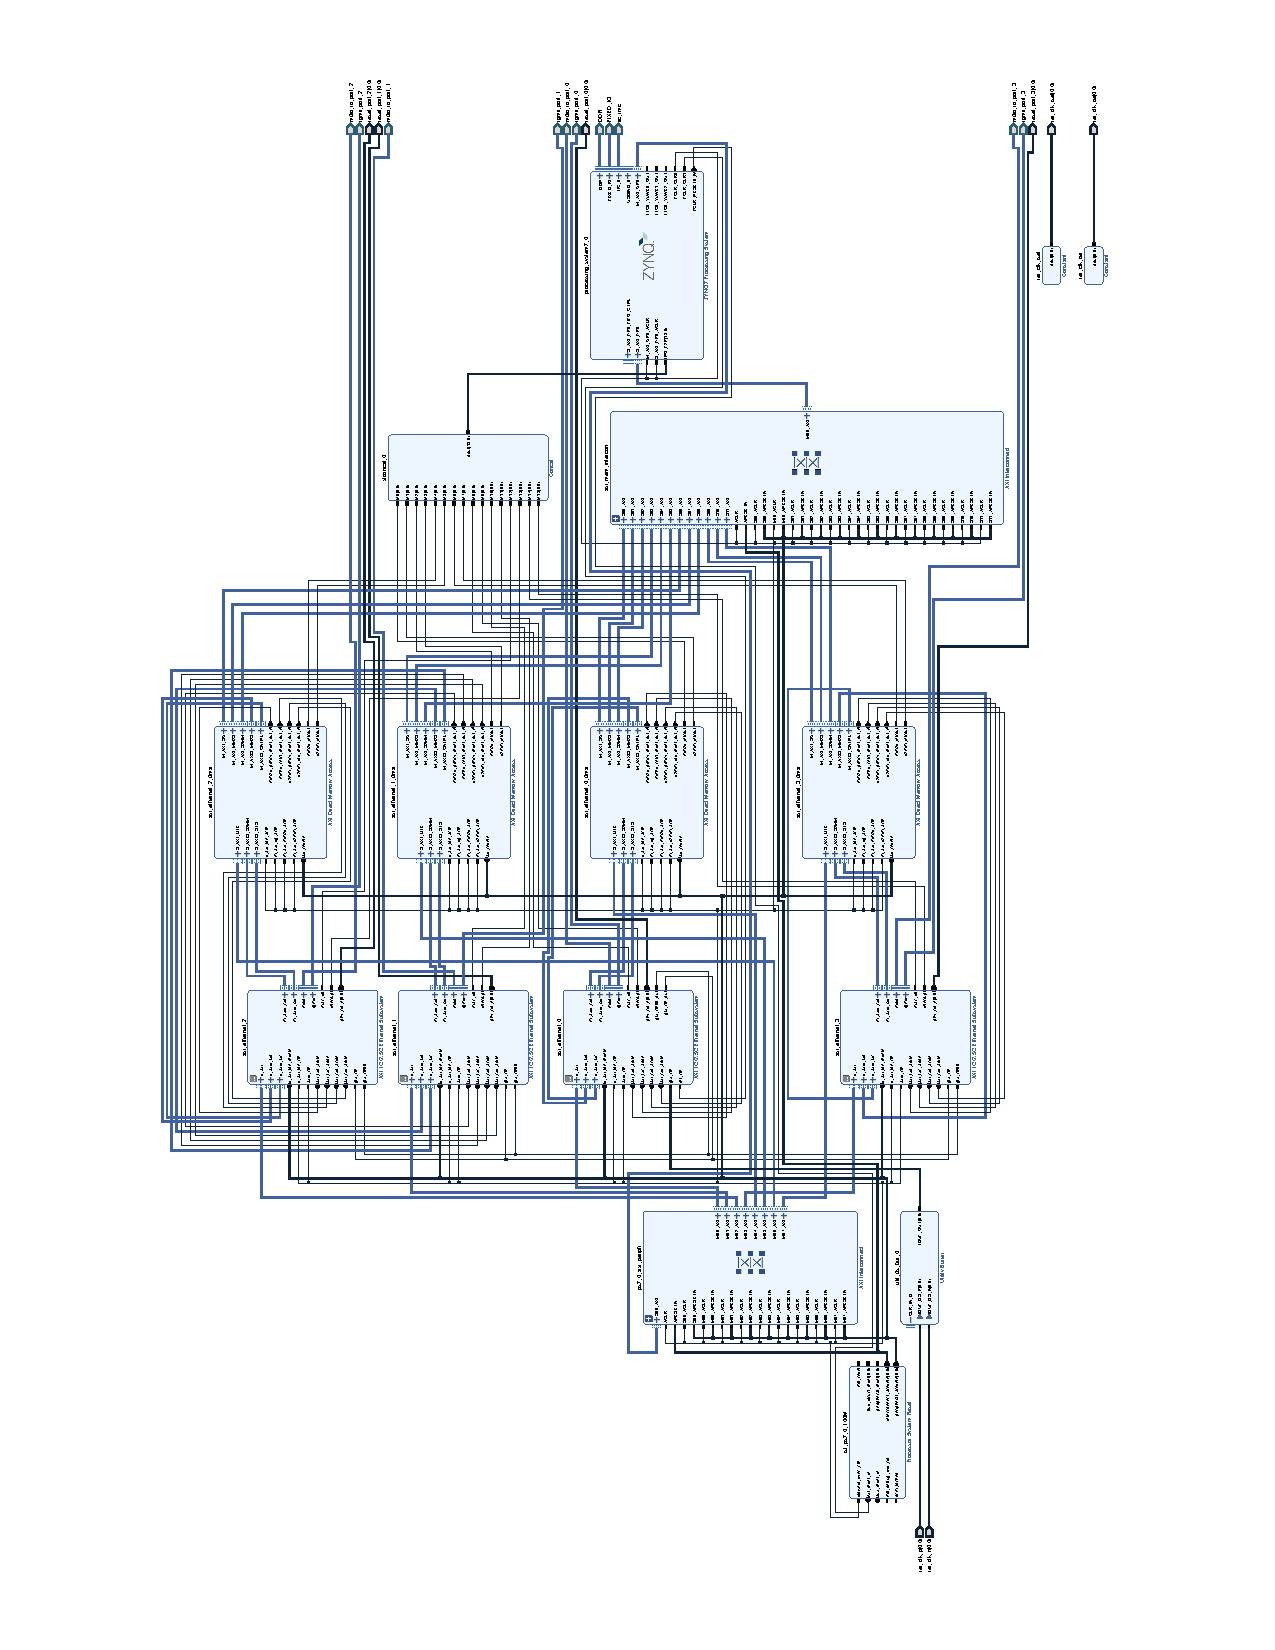
\includepdf[pages=-]{./PDFs/zedboard-axieth.pdf}


\end{document}
